\documentclass[11pt,a4paper]{article}
\usepackage{amsmath}
\usepackage{amsfonts}
\usepackage{amssymb}
\usepackage[utf8]{inputenc}
\usepackage[polish]{babel}
\usepackage[T1]{fontenc}
\usepackage{graphicx}
\usepackage{tikz}
%\usepackage{gensymb}
\usetikzlibrary{calc,through,backgrounds,positioning,fit}
\usetikzlibrary{shapes,arrows,shadows}
 
\author{Krzszystof stasiowski}
\begin{document}
\begin{figure}
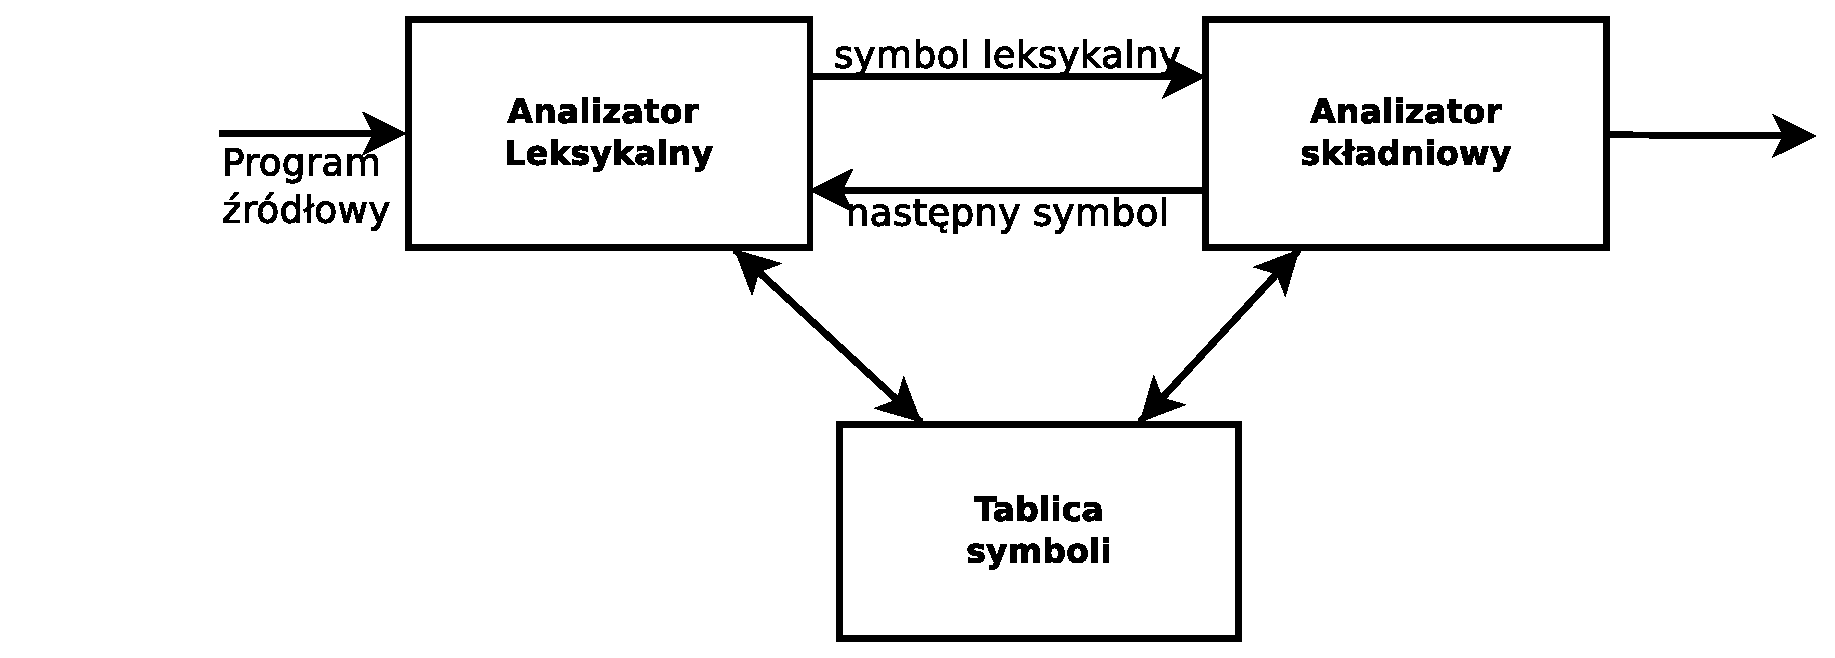
\includegraphics[width=\textwidth]{Diagram1.eps}
\end{figure}
\begin{figure}
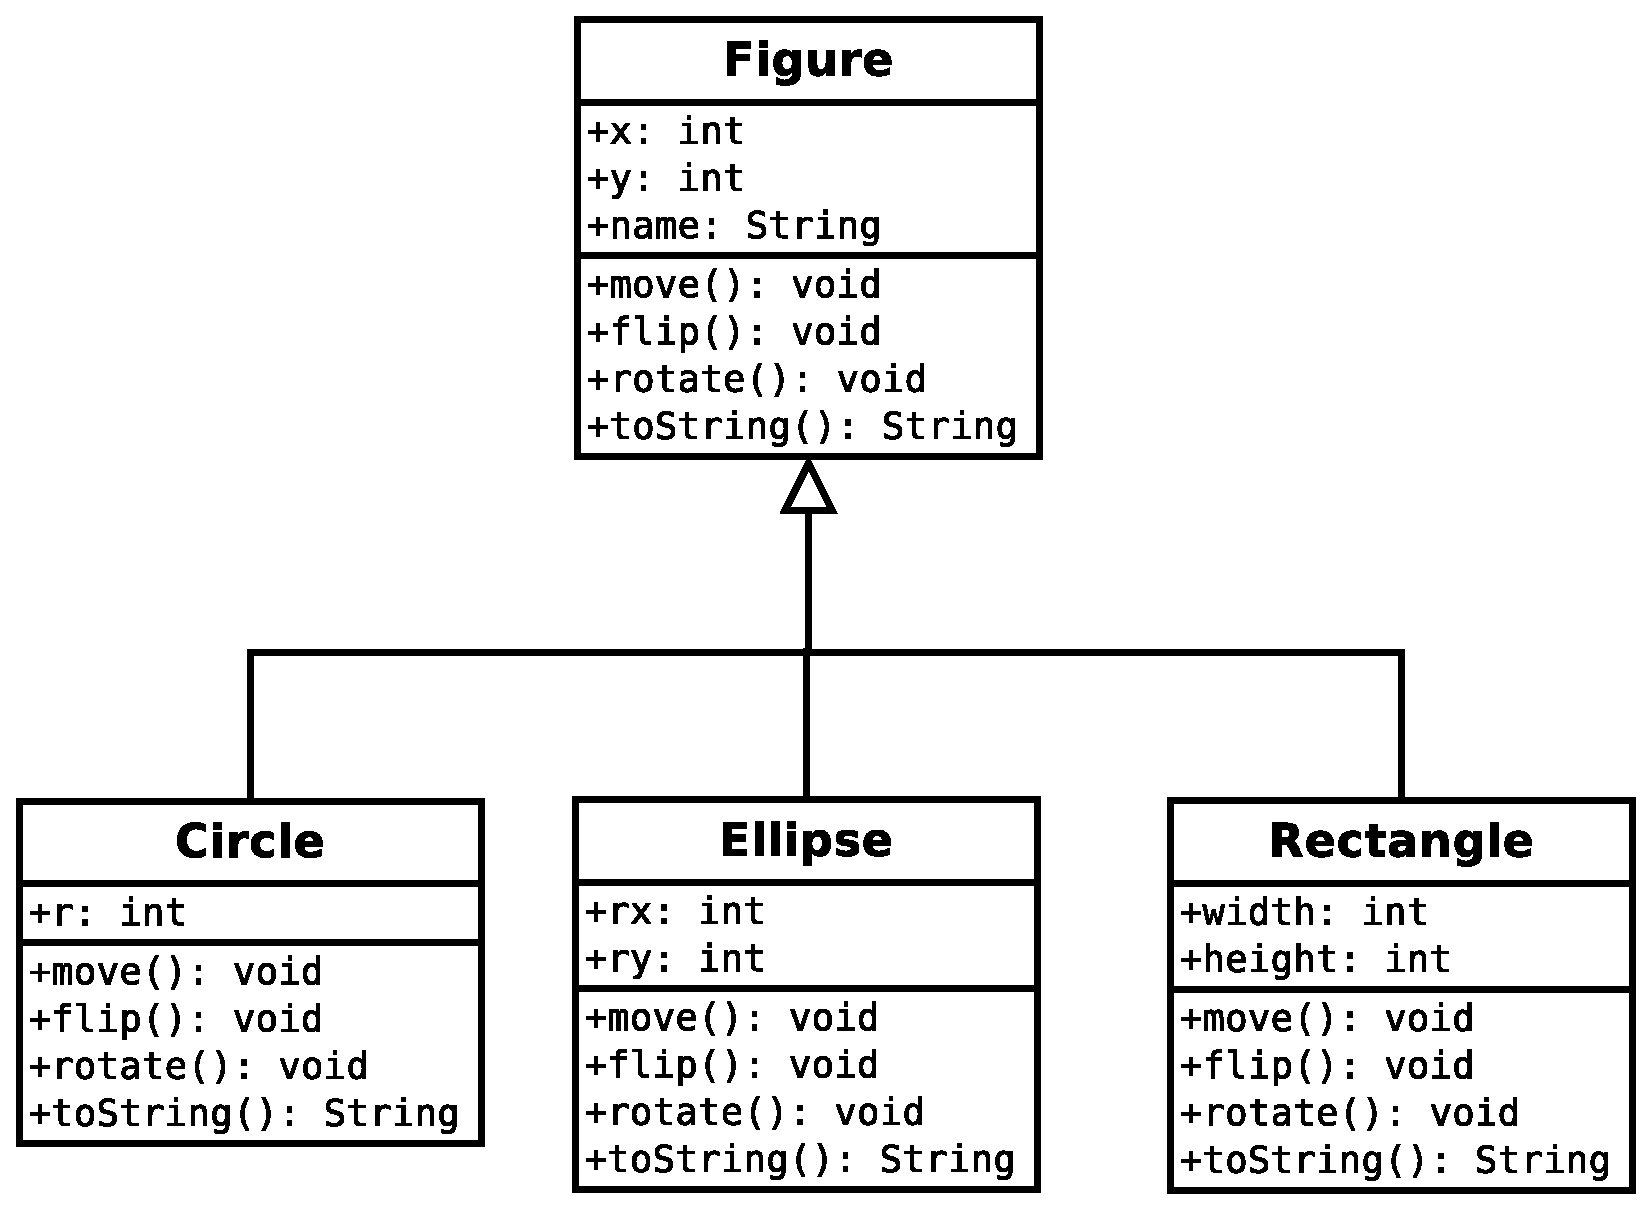
\includegraphics[width=\textwidth]{Diagram2.eps}
\end{figure}

\begin{figure}[!htb]
\centering
\begin{tikzpicture}
\node at (-0.1,0) {\includegraphics[scale=0.7]{f1.eps}};
\node at (5.6,-1.5) {$f(x) = \sin(x)$};
\node at (5.6,1.5) {$g(x) = \cos(x)$};
\node at (1.2,0.5) {$h(x) = \frac{\sin(x)}{2}$};
\end{tikzpicture}
\caption{Wykresy funkcji -tikz+xfig}
\label{fig:funkcje}
\end{figure}
\begin{figure}[!htb]
\centering
\begin{tikzpicture}
\node at (0,0) {\includegraphics[trim={90pt 350pt 90pt 350pt},clip,scale=0.7]{f1d.pdf}};
\node at (5.6,-1.5) {$f(x) = \sin(x)$};
\node at (5.6,1.5) {$g(x) = \cos(x)$};
\node at (2,1) {$h(x) = \frac{\sin(x)}{2}$};
\draw[->] (0,-2) to (0,2);
\draw[->] (-5,0) to (5,0);

\end{tikzpicture}
\caption{Wykresy funkcji -tikz}
\label{fig:funkcje2}
\end{figure}

\begin{figure}[!htb]
\centering
\begin{tikzpicture}[scale=1,inner sep=0.4mm]
\coordinate (O) at (0,0);
\coordinate (A) at (-75:2cm);
\coordinate (B) at (85:2cm);
\fill[fill=green,draw=gray] (O) --  (A) arc (-75:85:2cm)  -- cycle;

\node at (A) [circle,fill=black!80!white] {};
\node at (O) [circle,fill=black!80!white] {};
\node at (B) [circle,fill=black!80!white] {};
\node at (A) [above left=3pt] {$A$};
\node at (B) [below left=3pt] {$B$};
\node at (O) [left=2pt] {$O$};
\node at (O) [right=2pt] {$\alpha=160^{\circ}$};
%gensymb 160\degree
\draw (O) circle(2cm);

\end{tikzpicture}
\caption{okrąg-tikz}
\label{fig:okr}
\end{figure}

\begin{figure}[!htb]
\centering
\begin{tikzpicture}[scale=1,inner sep=0.4mm]
\coordinate (A) at  (1.6, 1, 1);
\coordinate (B) at  (3, 1, 1);
\coordinate (C) at  (3, 2, 1);
\coordinate (D) at  (1.6, 2, 1);

\coordinate (E) at  (1.6, 1, 3);
\coordinate (F) at  (3, 1, 3);
\coordinate (G) at  (3, 2, 3);
\coordinate (H) at  (1.6, 2, 3);

\coordinate (-C) at  (0, 2, 1);
\coordinate (-B) at  (0, 1, 1);
\coordinate (-G) at  (0, 2, 3);
\coordinate (-F) at  (0, 1, 3);

\coordinate (O) at  (0, 0, 0) ;
\coordinate (X) at  (3, 0, 0) ;
\coordinate (Y) at  (0, 3, 0) ;
\coordinate (Z) at  (0, 0, 4) ;
\coordinate (YZ) at  (0, 3, 4) ;



\draw[color=gray!80!red,fill=white!80!red] (O)--(0,2.7,0)--(0,2.7,3.5)--(0,0,3.5)--cycle;
\draw[thick,-latex] (O) -- (X);
\draw[thick,-latex] (O) -- (Y);
\draw[thick,-latex] (O) -- (Z);

\draw[thick] (E) -- (F) -- (G) -- (H) --cycle;
\draw[dashed] (A) -- (E);
\draw 		  (B) -- (F);
\draw (G) -- (C);
\draw (C) -- (D);
\draw (D) -- (H);
\draw (H) --(G);
\draw[dashed] (A) -- (B);
\draw (B) --(C) --(D);
\draw[dashed] (D)--(A);
\draw[dashed,color=red] (D)--(A);

\draw[color=red] (-B) -- (-C) -- (-G) -- (-F) --cycle;
\draw[dashed,color=red] (-B)--(A);
\draw[dashed,color=red] (-C)--(D);
\draw[dashed,color=red] (-G)--(H);
\draw[dashed,color=red] (-F)--(E);


\node at (X)[right=2pt] {$x$};
\node at (Y)[above=2pt] {$y$};
\node at (Z)[below left=2pt] {$z$};
\end{tikzpicture}
\caption{okrąg-tikz}
\label{fig:okr}
\end{figure}


\begin{figure}[!htb]
\centering
\begin{tikzpicture}[scale=1,inner sep=0.4mm]
\coordinate (P) at (0,1.5,0);
\coordinate (Q) at (0,0,0);
\coordinate (-Q) at (0,-1.2,0);
\coordinate (--Q) at (0,-1.6,0);




\draw[fill=white!80!red,color=white!80!red] (-3,0,-3)--(-3,0,3)--(3,0,3)--(3,0,-3)--cycle;
\node at (-3,0,3)[above=2pt] {$\pi$};
\node at (P)[circle,fill=gray]{};
\node at (P)[right=2pt]{$P(x_0,y_0,z_0)$};
\node at (0,2,0)[above left=2pt]{$l$};
\node at (Q)[circle,fill=gray]{};
\node at (Q)[right=2pt]{$Q(x_1,y_1,z_1)$};
\node at (0,1,0)[left=2pt]{$d$};
\node at (-Q)[right=2pt]{$\downarrow \textbf{n} = \left[a,b,c\right]$};


\draw[color=gray,very thick] (Q)--(P)--++(0,0.5,0) (--Q)--(-Q);
\draw[dashed,very thick] (-Q)--(Q);

\end{tikzpicture}
\caption{okrąg-tikz}
\label{fig:okr}
\end{figure}


\end{document}